\chapter{ATLAS}
\label{chap:ATLAS}

In this Chapter the ATLAS Pixel detector will be discussed, with a special focus on radiation
 damage. 
After a short introduction to the Large Hadron Collider (LHC) Physics program in 
Section~\ref{sec:LHCPhysics}, the ATLAS detector, one of the experiments at the LHC, will be 
presented (Section~\ref{sec:ATLASDetector}). Particular emphasis will be devoted to the 
the ATLAS Pixel Detector (Section~\ref{sec:ATLASPixelDetector}), before moving to the 
core of this Chapter - Section~\ref{sec:digitizer} -
 where the modelization of the radiation damage to the ATLAS Pixel 
Detector will be discussed. Finally, the impact of Radiation Damage on Higgs Analysis 
will be presented in Section~\ref{sec:raddamHiggs}; this is a study case that is in 
perspective very important given the excellent luminosity performance of LHC as we write.

\section{LHC Physics}
\label{sec:LHCPhysics}
Understanding the nature of electroweak symmetry breaking, and in particular  specifically 
deciphering the Higgs mechanism, is the main goal~\cite{Plehn:2009nd} of the ATLAS~\cite{AtlasDetector} and 
CMS~\cite{CMSDetector} experiments at the LHC~\cite{LHCMachine}. 
As already mentioned in Chapter~\ref{chap:context}
the two collaborations have both observed a boson compatible with the SM Higgs in 2012; 
since then the nature of that particle and its coupling to fundamental SM bosons and fermions 
keep being pursued.  Recently ATLAS reported evidence of $H\to\b\b$ decay~\cite{ATLASHbb2017} 
when produced in association with a $W$ or $Z$ boson; the CMS collaboration announced 
the first observation of Higgs boson decays to $\tau$ leptons~\cite{CMSHtautau2017}. 
The search for the Higgs boson decaying to second generation fermions is next on the 
agenda of the ATLAS and CMS collaborations (example:~\cite{ATLASHmumu2017}).

For the search of Higgs boson decaying to second generation fermions, for other Higgs sector 
studies, and for many New Physics (NP) scenarios not only outstanding tracking and vertexing of charged particles are needed but  excellent reconstruction of jets is mandatory  too. 
To achieve the highest possible performance tracker information should be exploited at maximum 
together with calorimeter. 
The chief advantages of integrating tracking and calorimetric information into one hadronic reconstruction
step are~\cite{ATLASParticleFlow}:

\begin{itemize}
\item the momentum resolution of the tracker is significantly better than the energy resolution of the
calorimeter for low-energy charged particles
\item the angular resolution of a single charged particle, reconstructed using the tracker is much better
than that of the calorimeter
\item better association of low $p_T$ charged particles to the right jet
\item better association to the correct production vertex so important reduction of degradation due to pile-up  
\end{itemize}

It is clear that the ATLAS tracking and vertexing detector, {\it i.e. the Inner Detector} is of the uttermost importance for all
the searches and studies of ATLAS.

\section{The ATLAS Detector}
\label{sec:ATLASDetector}

\section{The ATLAS Pixel Detector}
\label{sec:ATLASPixelDetector}


\begin{figure}[!htbp]
\centering
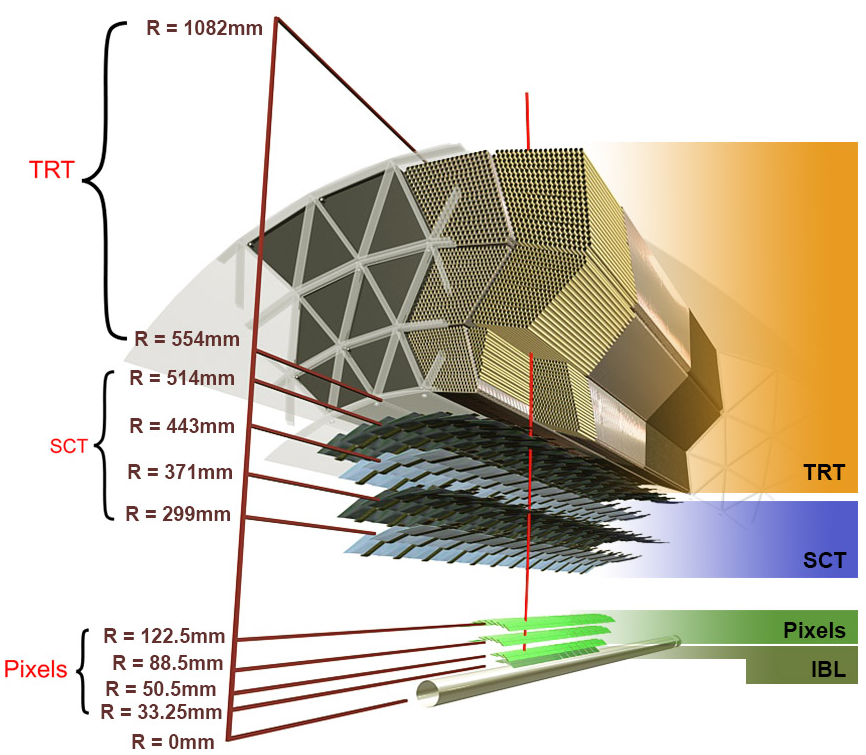
\includegraphics[width=0.5\textwidth]{ATLAS_ID.png}
\caption{\label{fig:ATLASID}Schematic view of the  ATLAS Inner Detector (ID), including the new Insertable B-Layer (IBL). (After~\cite{Potamianos:2016ptf})}
\end{figure}


\section{Radiation Damage to the ATLAS Pixel Detector}
\label{sec:digitizer}

\section{Impact of Radiation Damage on Higgs Analysis}
\label{sec:raddamHiggs}